\hypertarget{menu_8h}{
\section{menu.h File Reference}
\label{menu_8h}\index{menu.h@{menu.h}}
}
definition of the polynomial menu system 

{\tt \#include \char`\"{}poly.h\char`\"{}}\par
{\tt \#include \char`\"{}InputValidator.h\char`\"{}}\par
{\tt \#include $<$iostream$>$}\par
{\tt \#include $<$vector$>$}\par
{\tt \#include $<$utility$>$}\par


Include dependency graph for menu.h:\nopagebreak
\begin{figure}[H]
\begin{center}
\leavevmode
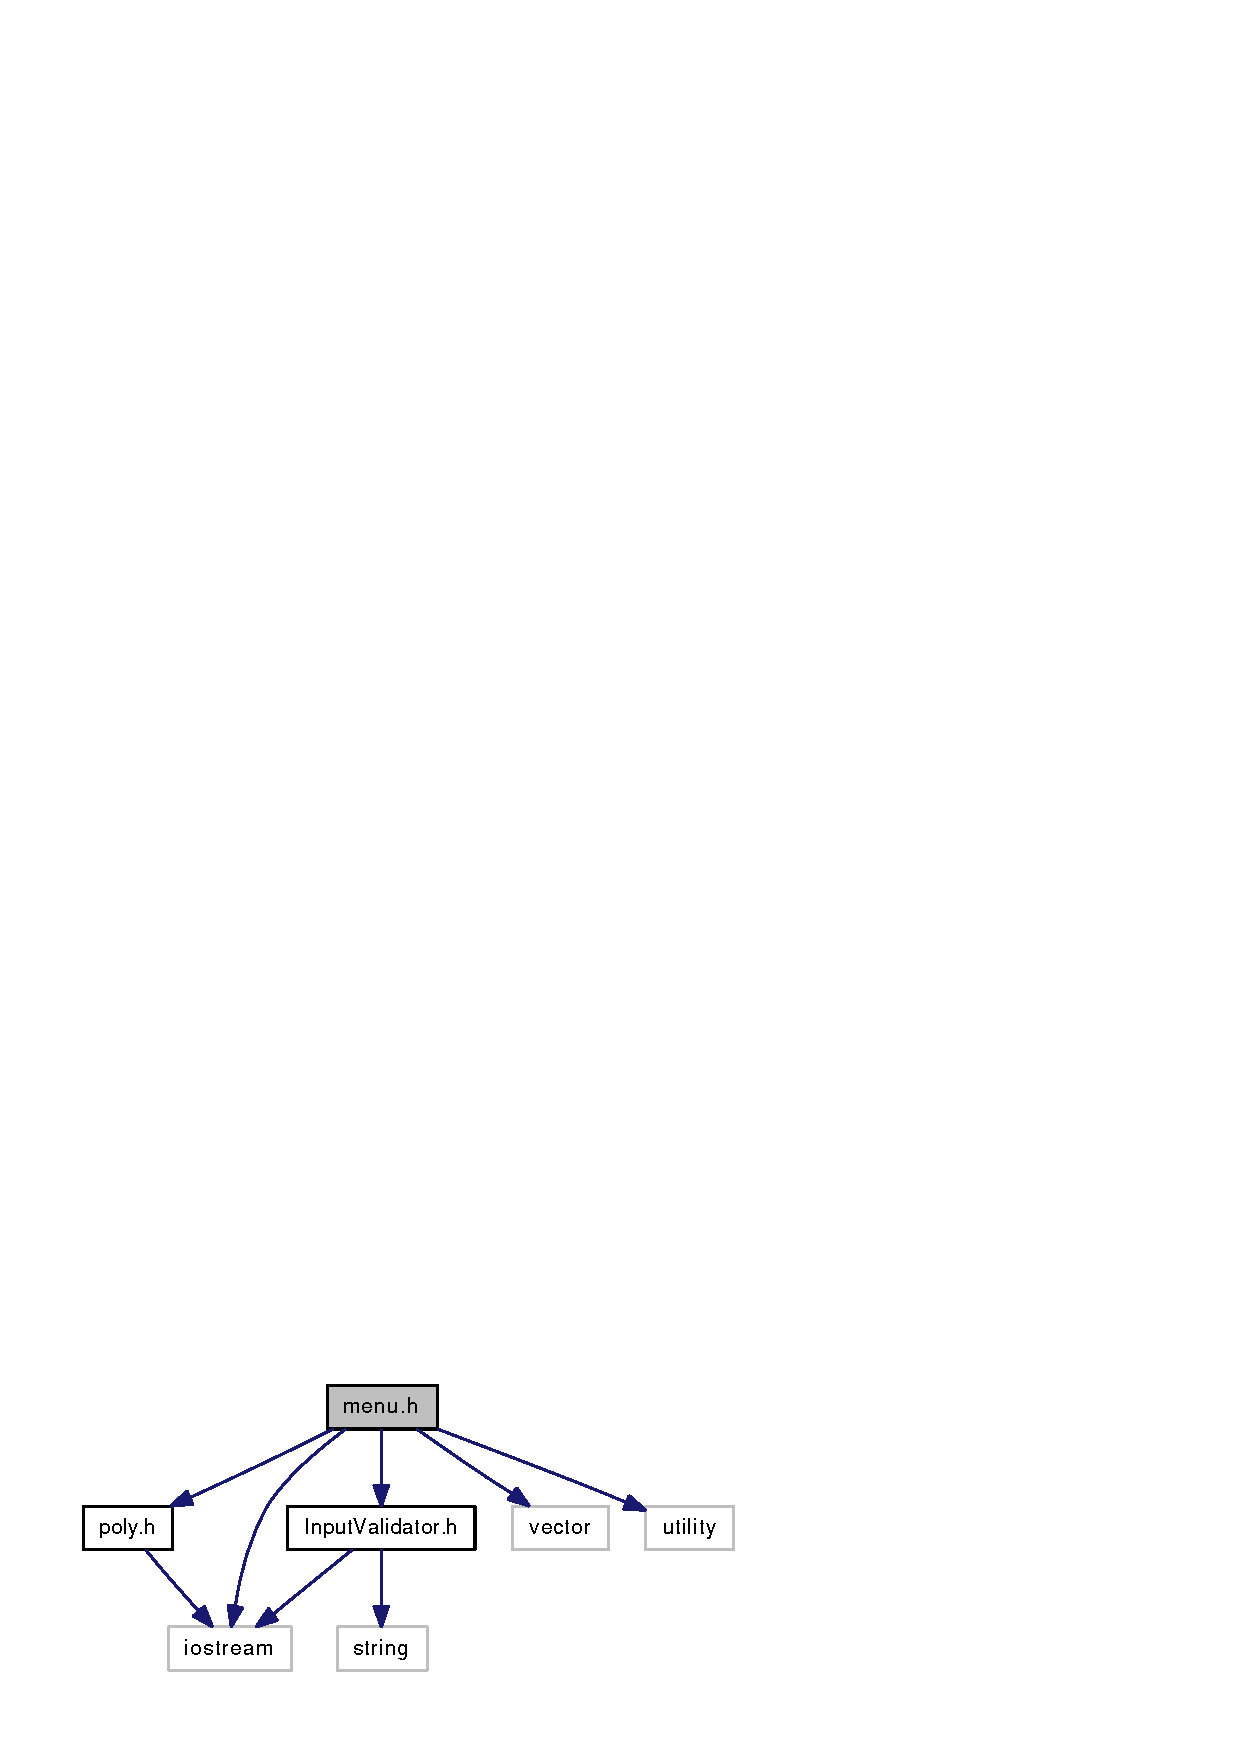
\includegraphics[width=178pt]{menu_8h__incl}
\end{center}
\end{figure}


This graph shows which files directly or indirectly include this file:\nopagebreak
\begin{figure}[H]
\begin{center}
\leavevmode
\includegraphics[width=86pt]{menu_8h__dep__incl}
\end{center}
\end{figure}
\subsection*{Classes}
\begin{CompactItemize}
\item 
class \hyperlink{classPolynomialMenu}{PolynomialMenu}
\begin{CompactList}\small\item\em The main program logic, contains a vector of Polynomials, means to generate them, means to add and multiply existing polynomials, handles user input/output, and displays the menu and the polynomials in the vector. \item\end{CompactList}\end{CompactItemize}


\subsection{Detailed Description}
definition of the polynomial menu system 

\begin{Desc}
\item[Author:]Daniel Uber \end{Desc}


Definition in file \hyperlink{menu_8h-source}{menu.h}.